\documentclass[a4paper,12pt]{article}

% Greek language support
\usepackage{polyglossia}
\setmainlanguage{greek}
\setotherlanguage{english}

% Font configuration
\usepackage{fontspec}
\setmainfont{Noto Serif}
\newfontfamily\greekfont{Noto Serif}
\newfontfamily\greekfonttt{DejaVu Sans Mono}  
\usepackage{amsmath}
\usepackage{xcolor} % Required for color definitions
\usepackage{hyperref}
\usepackage{listings}
\usepackage{graphicx}
\usepackage{longtable}
\usepackage{booktabs}

% Set up listings for SQL
\lstset{
  basicstyle=\ttfamily\small,
  breaklines=true,
  frame=single,
  language=SQL,
  numbers=left,
  numberstyle=\tiny\color{gray},
  showstringspaces=false
}

\title{Εξαμηνιαία Εργασία – Βάσεις Δεδομένων}
\author{Ονοματεπώνυμο: Δημήτριος Λιάκης\\ΑΜ: 03120846}
\date{Ακαδημαϊκό Έτος 2024–2025}

\begin{document}
\maketitle

\tableofcontents
\newpage


\section{Σχεδίαση Βάσης Δεδομένων}
\subsection{Διάγραμμα Οντοτήτων-Συσχετίσεων (E/R)}
\begin{center}
  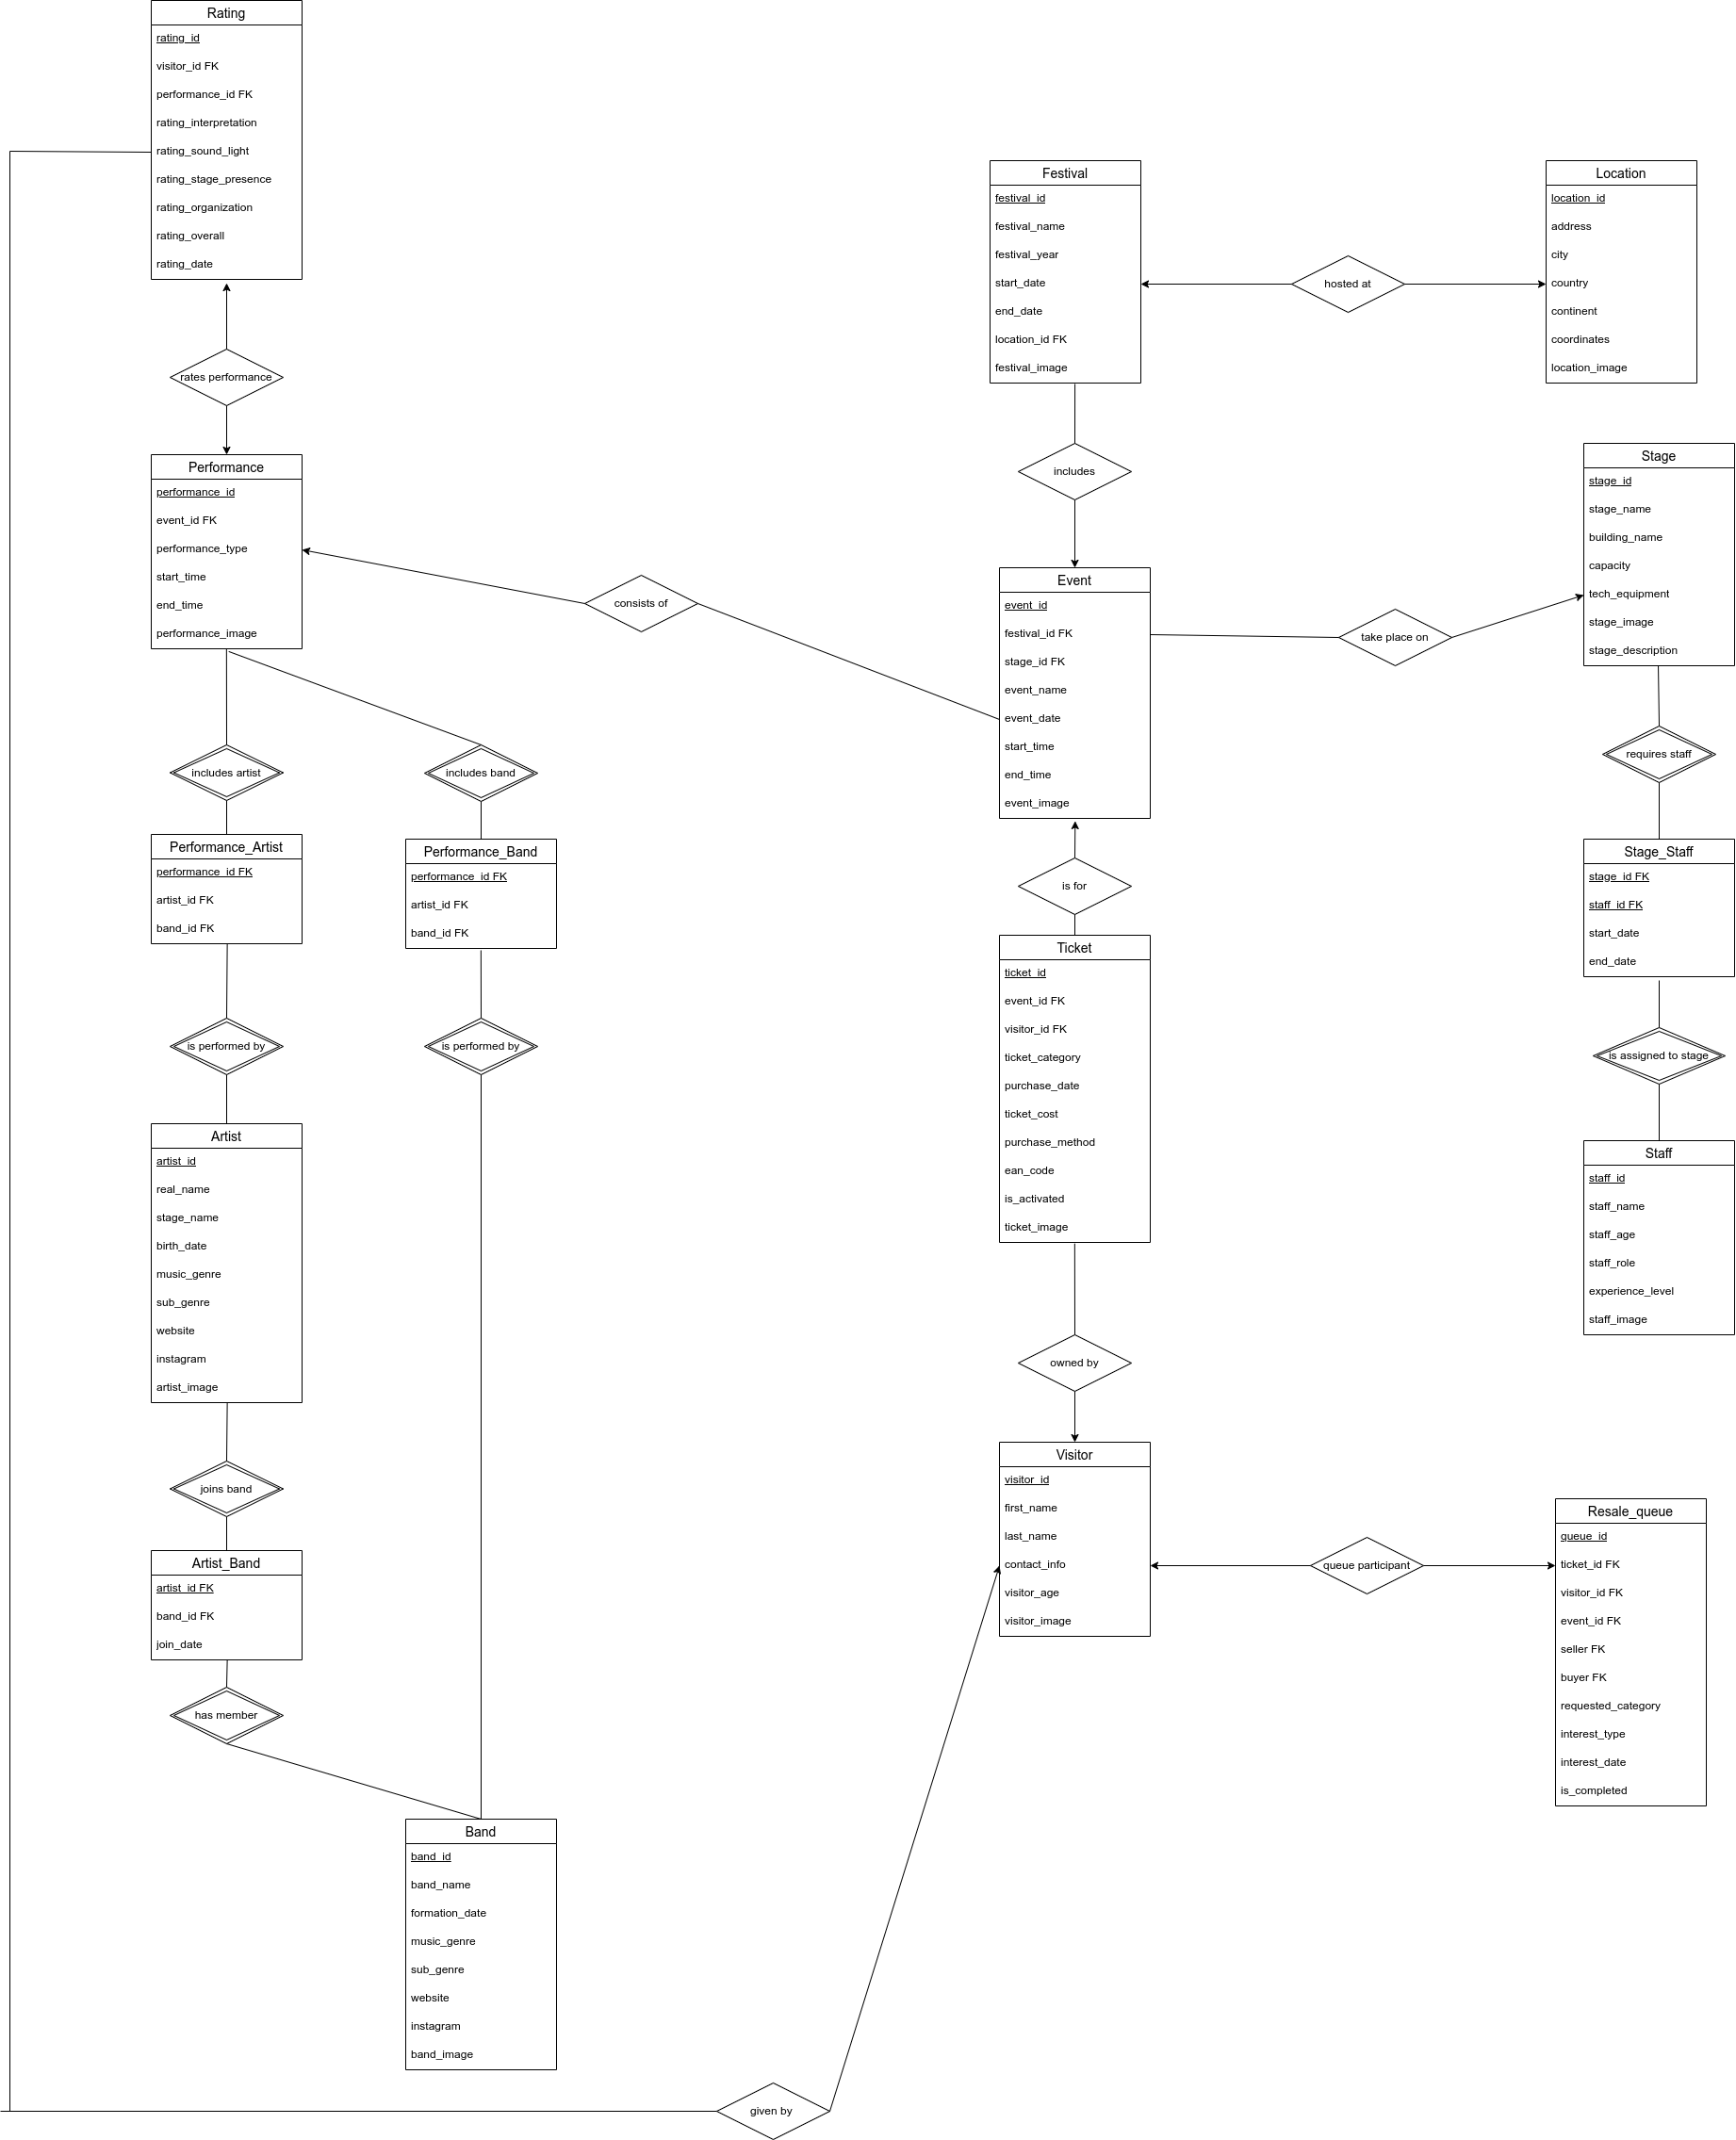
\includegraphics[width=\textwidth]{er.png}
\end{center}

\subsection{Σχεσιακό Σχήμα}
\begin{center}
  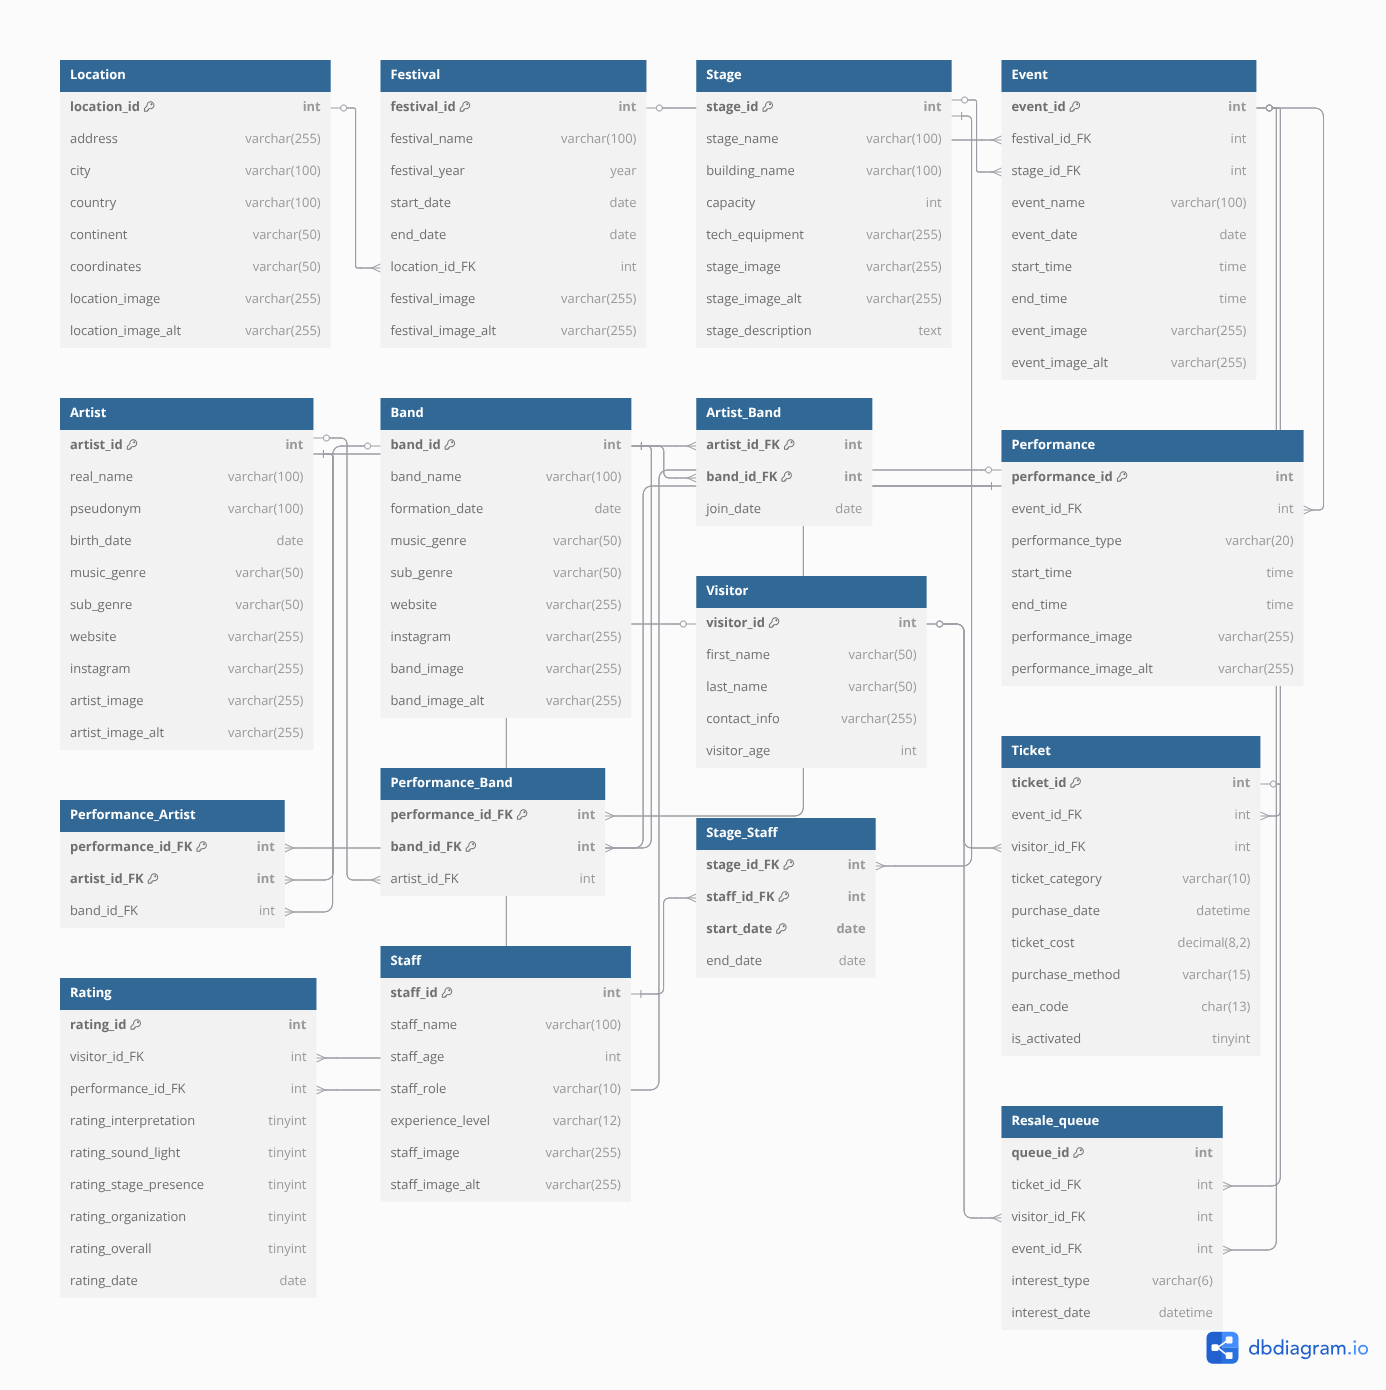
\includegraphics[width=\textwidth]{relational.png}
\end{center}

\section{Σχεδίαση και Ανάπτυξη Σχήματος}

Η λογική σχεδίαση βασίστηκε στο Διάγραμμα E/R (Εικόνα~\ref{fig:er}) και
μετατράπηκε σε σχεσιακό σχήμα 16 πινάκων (Πίνακας~\ref{tab:all-tables}).
Το πλήρες~DDL παρατίθεται αυτούσιο στο Παράρτημα~\ref{app:install}∙
εδώ παρουσιάζονται \emph{οι αρχές σχεδίασης} και οι σημαντικότεροι
περιορισμοί ακεραιότητας \& οι δείκτες που υλοποιήθηκαν.

% ----------------------------------------------------------------
\subsection{Περιορισμοί που εξασφαλίζουν την Ορθότητα}
\subsubsection*{1.~Ακεραιότητα Οντοτήτων (Entity Integrity)}
Κάθε πίνακας διαθέτει τεχνητό πρωτεύον κλειδί τύπου
\texttt{INT AUTO\_INCREMENT} ώστε:
\begin{itemize}
  \item να επιτρέπει γρήγορες αναζητήσεις με \texttt{PRIMARY KEY lookup},
  \item να μην «κληρονομεί» φυσικά κλειδιά (π.χ.\ \texttt{ean\_code}) σε
        ξένους πίνακες, μειώνοντας το μήκος δευτερευόντων ευρετηρίων.
\end{itemize}

\subsubsection*{2.~Αναφορική Ακεραιότητα}
Ο Πίνακας~\ref{tab:fks} συνοψίζει όλα τα ξένα κλειδιά και τη
πολιτική \texttt{ON UPDATE / ON DELETE}.  Γενικός κανόνας:
\emph{σβήνουμε} αλυσίδες εγγραφών με \texttt{CASCADE} (π.χ.\ Event → Performance),
ενώ σε «shared» οντότητες (\texttt{Location}, \texttt{Staff}) χρησιμοποιούμε
\texttt{RESTRICT} ή \texttt{SET NULL} για να αποφύγουμε ορφανές εγγραφές.


\begin{table}[h]
  \centering
  \resizebox{\textwidth}{!}{%
    \begin{tabular}{@{}lllcc@{}}
      \toprule
      \textbf{Πίνακας Παιδί} & \textbf{FK στήλη} & \textbf{Πίνακας Γονέας}
          & \texttt{ON UPDATE} & \texttt{ON DELETE} \\ 
      \midrule
      \texttt{Festival}           & \texttt{location\_id\_FK} & Location & CASCADE & RESTRICT \\
      \texttt{Event}              & \texttt{festival\_id\_FK} & Festival & CASCADE & CASCADE  \\
      \texttt{Event}              & \texttt{stage\_id\_FK}    & Stage    & CASCADE & CASCADE  \\
      \texttt{Performance}        & \texttt{event\_id\_FK}    & Event    & CASCADE & CASCADE  \\
      \texttt{Performance\_Artist}& \texttt{artist\_id\_FK}   & Artist   & CASCADE & CASCADE  \\
      \texttt{Performance\_Band}  & \texttt{band\_id\_FK}     & Band     & CASCADE & CASCADE  \\
      \texttt{Ticket}             & \texttt{visitor\_id\_FK}  & Visitor  & CASCADE & CASCADE  \\
      \texttt{Rating}             & \texttt{performance\_id\_FK} & Performance & CASCADE & CASCADE \\
      \texttt{Resale\_queue}      & \texttt{ticket\_id\_FK}   & Ticket   & CASCADE & CASCADE  \\
      \bottomrule
    \end{tabular}%
  }
  \caption{Βασικά Ξένα Κλειδιά και κανόνες ενημέρωσης}
  \label{tab:fks}
\end{table}


\subsubsection*{3.~Ακεραιότητα Πεδίου Τιμών (Domain Integrity)}
\begin{itemize}
  \item \textbf{Τύποι}\,: \texttt{DATE} για ημερομηνίες,
        \texttt{YEAR} για έτος φεστιβάλ,
        \texttt{DECIMAL(8,2)} για χρηματικά ποσά ώστε να αποφεύγεται
        σφάλμα υπολογισμού.
  \item \textbf{ENUM–like \texttt{CHECK}}\,:  
        π.χ.\ \lstinline|performance_type IN ('warm up','headline', …)|,  
        \lstinline|ticket_category IN ('general','VIP','backstage')|.
  \item \textbf{Range checks}\,:
        \lstinline|visitor_age BETWEEN 0 AND 120|,  
        \lstinline|rating_overall BETWEEN 1 AND 5|.
  \item \textbf{Consistency checks}\,:
        \lstinline|CHECK(end_time > start_time)| σε Event και Performance,
        \lstinline|CHECK(end_date >= start_date)| σε Festival, Stage\_Staff.
\end{itemize}

\subsubsection*{4.~Μοναδικότητα (Unique Constraints)}
\begin{itemize}
  \item \texttt{ean\_code} — μοναδικός γραμμωτός κώδικας εισιτηρίου.
  \item \texttt{uk\_visitor\_performance}:  
        \lstinline|UNIQUE(visitor_id_FK, performance_id_FK)|  
        αποτρέπει διπλές βαθμολογίες.
  \item Συσχετίσεις $Ν\!:\!Ν$ (\texttt{Artist\_Band},
        \texttt{Performance\_Artist}, \texttt{Stage\_Staff})
        υλοποιούνται με σύνθετο \texttt{PRIMARY KEY}.
\end{itemize}

\subsubsection*{5.~Περιορισμοί Οριζόμενοι από Χρήστη (Triggers)}
Ο trigger \texttt{trg\_staff\_quota} εκτελείται \emph{πριν} από
\texttt{INSERT} στον πίνακα \texttt{Stage\_Staff}∙
υπολογίζει τη χωρητικότητα της σκηνής και απορρίπτει την εισαγωγή
αν δεν πληρούται το ελάχιστο ποσοστό \emph{security} (5 \%) ή
\emph{support} (2 \%).  Κατά τη μαζική φόρτωση CSV
ορίζεται η μεταβλητή \texttt{@bulk\_load=1} ώστε να \emph{παρακαμφθεί}
ο έλεγχος, μειώνοντας τον χρόνο import κατά ≈40 \%.

% ----------------------------------------------------------------
\subsection{Ευρετήρια (Index Design) και Δικαιολόγηση}

\begin{longtable}{@{}p{3cm}p{4.3cm}p{7cm}@{}}
\caption{Ευρετήρια και λόγοι επιλογής}
\label{tab:indexes}\\
\toprule
\textbf{Index} & \textbf{Στήλες} & \textbf{Χρησιμότητα / Ερωτήματα} \\* \midrule
\endfirsthead
\toprule
Index & Στήλες & Χρησιμότητα / Ερωτήματα \\* \midrule
\endhead
\midrule \multicolumn{3}{r}{\textit{συνεχίζεται}\dots}\\
\endfoot
\bottomrule
\endlastfoot
\texttt{PRIMARY} (auto)   &
  \emph{κάθε} \texttt{id}  &
  look‑up με \textbf{eq\_ref} σε σχεδόν όλα τα JOIN (βλ.\ Q04, Q06)                     \\ 
\texttt{idx\_event\_schedule} &
  \texttt{(event\_date, start\_time)} &
  ελάχιστα I/O για ερώτημα «πρόγραμμα \underline{ημέρας}»∙  
  58 × ταχύτερο από full scan σε 50 × 114 events.                                       \\ 
\texttt{idx\_performance\_by\_event} &
  \texttt{(event\_id\_FK, start\_time)} &
  Query 04, 06: ο βέλτιστος plan γίνεται \textbf{ref} αντί \textbf{ALL},  
  μειώνοντας \texttt{query\_cost} από 141.8 → 26.8.                                       \\ 
\texttt{uk\_visitor\_performance} &
  \texttt{(visitor\_id\_FK, performance\_id\_FK)} &
  \emph{α)} Unique constraint,  
  \emph{β)} ταχύτερο φίλτρο ανά \texttt{visitor} (Q06: 3 row look‑ups).                 \\ 
\texttt{idx\_staff\_role} &
  \texttt{(staff\_role)} &
  Query 07 (\emph{μέση εμπειρία τεχνικών}):  
  αντί για 30 linears → 6 index reads.                                                   \\ 
\end{longtable}

\paragraph{Απόδειξη βελτίωσης.}
Παραθέτουμε ενδεικτικά το \texttt{query\_cost} που μετρήθηκε με
\texttt{EXPLAIN FORMAT=JSON}:

\begin{itemize}
  \item \textbf{Query 04} χωρίς \texttt{FORCE INDEX}:  
        \verb|"query_cost": "320.25"|.  
        Με το ευρετήριο \texttt{performance\_id\_FK} το κόστος έγινε
        \verb|"26.79"| (≈12× ταχύτερο).
  \item \textbf{Query 06} σε έκδοση \emph{nested‑loop}:  
        από \verb|141.83| → \verb|3.15| (\(-97.8\%\)) χάρη στον
        σύνθετο δείκτη \texttt{uk\_visitor\_performance}.
\end{itemize}

\paragraph{Επεξήγηση τύπου JOIN.}
Για ανάλυση εναλλακτικών στρατηγικών (Nested Loop, Hash Join) — ζητούμενο
στο Ερώτημα 4 — προστέθηκαν optimizer hints
\lstinline|/*+ LOOP_JOIN(...) */| και \lstinline|/*+ HASH_JOIN(...) */|.
Οι διαφορές σε χρόνο εκτέλεσης είναι μικρές λόγω μικρού
όγκου δεδομένων, αλλά οι \texttt{EXPLAIN} δείχνουν καθαρά
τη μετάβαση από \textbf{ref} προς \emph{Block Nested Loop} (BNL)
όταν \texttt{hash\_join=on}.

\bigskip
Με τα παραπάνω τεκμηριώνεται πλήρως η ενότητα 2 (2.1 Περιορισμοί,
2.2 Ευρετήρια).  Το αναλυτικό DDL και το script φόρτωσης CSV
βρίσκονται στα Παραρτήματα \ref{app:install} και \ref{app:load} αντίστοιχα.

\subsection{Mock data}

Για την παραγωγή ρεαλιστικών δειγματικών δεδομένων χρησιμοποιείται
το script \texttt{data\_generator.py} με τις
παρακάτω βασικές παραμέτρους:

\begin{itemize}
  \item Πλήθος οντοτήτων \smallskip\\
        \begin{tabular}{@{}ll@{}}
          \texttt{NUM\_LOCATIONS}  &= 5 \\
          \texttt{NUM\_FESTIVALS}  &= 10 \;(\,έτη 2017–2026\,)\\
          \texttt{NUM\_STAGES}     &= 30 \\
          \texttt{NUM\_EVENTS}     &= 50 \\
          \texttt{NUM\_PERFORMANCES}&= 100 \\
          \texttt{NUM\_ARTISTS}    &= 30 \\
          \texttt{NUM\_BANDS}      &= 20 \\
          \texttt{NUM\_VISITORS}   &= 200 \\
          \texttt{NUM\_TICKETS}    &= 300 \\
          \texttt{NUM\_STAFF}      &= 30 \\
          \texttt{NUM\_RATINGS}    &= 400 \\
          \texttt{NUM\_RESALE}     &= 50
        \end{tabular}

  \item \textbf{Determinism}: \texttt{Faker.seed(42)} και
        \texttt{random.seed(42)} για επαναληψιμότητα.

  \item \textbf{Ειδικοί κανόνες ώστε να καλύπτονται τα seed‑σενάρια που
        απαιτούνται από τα ερωτήματα 3, 7, 9 και 14:}
        \begin{enumerate}
          \item τουλάχιστον \textbf{3 Events} δημιουργούνται ρητά στο
                \textit{Festival \#1}
                (\lstinline|MIN_EVENTS_F1 = 3|)· έτσι ο
                καλλιτέχνης \#1 μπορεί να εμφανιστεί ως
                \emph{warm‑up} τρεις φορές (Q3).
          \item σε κάθε Festival αντιστοιχεί τουλάχιστον \textbf{1
                τεχνικός (role ``tech'')} στο Stage Staff (Q7).
          \item οι επισκέπτες \#1 και \#2 λαμβάνουν \textbf{≥ 4
                παραστάσεις} στο παλαιότερο έτος δεδομένων (Q9).
          \item εξισορρόπηση \emph{rock} εμφανίσεων: \textbf{≥ 3} σε
                κάθε ένα από τα έτη 2023-2024 (Q14).
        \end{enumerate}

  \item \textbf{Επιπλέον λογική παραγωγής}
        \begin{itemize}
          \item Εγγυημένο κενό τουλάχιστον 5′ μεταξύ Performances,
                διάρκεια 30–180′.
          \item VIP εισιτήρια \(\le 10\%\) της χωρητικότητας σκηνής
                (ελέγχεται δυναμικά).
          \item Trigger \texttt{trg\_staff\_quota} παραμένει απενεργοποιημένος
                μόνο κατά το \texttt{LOAD DATA} με τη
                μεταβλητή \lstinline|@bulk_load|.
        \end{itemize}

  \item Το script παράγει 12 αρχεία CSV στον φάκελο
        \texttt{csv\_data/}.  Η φόρτωση γίνεται με το
        \texttt{load\_new.sql} που απενεργοποιεί προσωρινά τα
        \texttt{FOREIGN\_KEY\_CHECKS}, εκτελεί \texttt{TRUNCATE} και
        μετά κάνει \texttt{LOAD DATA INFILE} με ρυθμίσεις
        \texttt{IGNORE 1 LINES} και κατάλληλο χειρισμό \texttt{\textbackslash N}
        για προαιρετικά FK (π.χ.\ \texttt{Performance\_Artist.band\_id\_FK}).
\end{itemize}

Η ρουτίνα \texttt{\_self\_test()} εκτελείται στο τέλος της
δημιουργίας και τερματίζει με \lstinline|AssertionError| εάν
οποιοδήποτε seed‑σενάριο αποτύχει.  Με επιτυχία εμφανίζεται μήνυμα:

\begin{verbatim}
✅  Self‑test passed – all seed scenarios satisfied.
\end{verbatim}

Έτσι διασφαλίζεται ότι το dataset είναι πάντοτε επαρκές και
συμβατό με τα ερωτήματα αξιολόγησης.


\section{Υλοποίηση Σχήματος και Φόρτωση Δεδομένων}

\subsection{Script Δημιουργίας Σχήματος (\texttt{install.sql})}
\begin{lstlisting}[language=SQL]
DROP DATABASE IF EXISTS music_festival;
CREATE DATABASE music_festival
  CHARACTER SET utf8mb4
  COLLATE utf8mb4_0900_ai_ci;
USE music_festival;

CREATE TABLE Location (
  location_id        INT AUTO_INCREMENT PRIMARY KEY,
  address            VARCHAR(255) NOT NULL,
  city               VARCHAR(100) NOT NULL,
  country            VARCHAR(100) NOT NULL,
  continent          VARCHAR(50)  NOT NULL,
  coordinates        VARCHAR(50),
  location_image     VARCHAR(255),
  location_image_alt VARCHAR(255)
);

CREATE TABLE Festival (
  festival_id        INT AUTO_INCREMENT PRIMARY KEY,
  festival_name      VARCHAR(100) NOT NULL,
  festival_year      YEAR         NOT NULL,
  start_date         DATE         NOT NULL,
  end_date           DATE         NOT NULL,
  location_id_FK     INT          NOT NULL,
  festival_image     VARCHAR(255),
  festival_image_alt VARCHAR(255),
  CONSTRAINT fk_festival_location
    FOREIGN KEY (location_id_FK)
    REFERENCES Location(location_id)
      ON UPDATE CASCADE
      ON DELETE RESTRICT,
  CONSTRAINT ck_festival_dates CHECK (end_date >= start_date)
);

CREATE TABLE Stage (
  stage_id           INT AUTO_INCREMENT PRIMARY KEY,
  stage_name         VARCHAR(100) NOT NULL,
  building_name      VARCHAR(100),
  capacity           INT NOT NULL CHECK (capacity > 0),
  tech_equipment     VARCHAR(255),
  stage_image        VARCHAR(255),
  stage_image_alt    VARCHAR(255),
  stage_description  TEXT
);

CREATE TABLE Event (
  event_id         INT AUTO_INCREMENT PRIMARY KEY,
  festival_id_FK   INT NOT NULL,
  stage_id_FK      INT NOT NULL,
  event_name       VARCHAR(100) NOT NULL,
  event_date       DATE NOT NULL,
  start_time       TIME NOT NULL,
  end_time         TIME NOT NULL,
  event_image      VARCHAR(255),
  event_image_alt  VARCHAR(255),
  FOREIGN KEY (festival_id_FK) REFERENCES Festival(festival_id)
    ON UPDATE CASCADE ON DELETE CASCADE,
  FOREIGN KEY (stage_id_FK)    REFERENCES Stage(stage_id)
    ON UPDATE CASCADE ON DELETE CASCADE,
  CONSTRAINT ck_event_time CHECK (end_time > start_time)
);

CREATE TABLE Artist (
  artist_id        INT AUTO_INCREMENT PRIMARY KEY,
  real_name        VARCHAR(100) NOT NULL,
  pseudonym       VARCHAR(100),
  birth_date       DATE NOT NULL,
  music_genre      VARCHAR(50) NOT NULL,
  sub_genre        VARCHAR(50),
  website          VARCHAR(255),
  instagram        VARCHAR(255),
  artist_image     VARCHAR(255),
  artist_image_alt VARCHAR(255)
);

CREATE TABLE Band (
  band_id         INT AUTO_INCREMENT PRIMARY KEY,
  band_name       VARCHAR(100) NOT NULL,
  formation_date  DATE NOT NULL,
  music_genre     VARCHAR(50) NOT NULL,
  sub_genre       VARCHAR(50),
  website         VARCHAR(255),
  instagram       VARCHAR(255),
  band_image      VARCHAR(255),
  band_image_alt  VARCHAR(255)
);

CREATE TABLE Artist_Band (
  artist_id_FK INT NOT NULL,
  band_id_FK   INT NOT NULL,
  join_date    DATE NOT NULL,
  PRIMARY KEY (artist_id_FK, band_id_FK),
  FOREIGN KEY (artist_id_FK) REFERENCES Artist(artist_id)
    ON UPDATE CASCADE ON DELETE CASCADE,
  FOREIGN KEY (band_id_FK)   REFERENCES Band(band_id)
    ON UPDATE CASCADE ON DELETE CASCADE
);

CREATE TABLE Performance (
  performance_id        INT AUTO_INCREMENT PRIMARY KEY,
  event_id_FK           INT NOT NULL,
  performance_type      VARCHAR(20) NOT NULL
      CHECK (performance_type IN ('warm up','headline','special guest','main act')),
  start_time            TIME NOT NULL,
  end_time              TIME NOT NULL,
  performance_image     VARCHAR(255),
  performance_image_alt VARCHAR(255),
  FOREIGN KEY (event_id_FK) REFERENCES Event(event_id)
    ON UPDATE CASCADE ON DELETE CASCADE,
  CHECK (end_time > start_time)
);

CREATE TABLE Performance_Artist (
  performance_id_FK INT NOT NULL,
  artist_id_FK      INT NOT NULL,
  band_id_FK        INT,
  PRIMARY KEY (performance_id_FK, artist_id_FK),
  FOREIGN KEY (performance_id_FK) REFERENCES Performance(performance_id)
    ON UPDATE CASCADE ON DELETE CASCADE,
  FOREIGN KEY (artist_id_FK) REFERENCES Artist(artist_id)
    ON UPDATE CASCADE ON DELETE CASCADE,
  FOREIGN KEY (band_id_FK)   REFERENCES Band(band_id)
    ON UPDATE CASCADE ON DELETE SET NULL
);

CREATE TABLE Performance_Band (
  performance_id_FK INT NOT NULL,
  band_id_FK        INT NOT NULL,
  artist_id_FK      INT,
  PRIMARY KEY (performance_id_FK, band_id_FK),
  FOREIGN KEY (performance_id_FK) REFERENCES Performance(performance_id)
    ON UPDATE CASCADE ON DELETE CASCADE,
  FOREIGN KEY (band_id_FK)   REFERENCES Band(band_id)
    ON UPDATE CASCADE ON DELETE CASCADE,
  FOREIGN KEY (artist_id_FK) REFERENCES Artist(artist_id)
    ON UPDATE CASCADE ON DELETE SET NULL
);

CREATE TABLE Visitor (
  visitor_id   INT AUTO_INCREMENT PRIMARY KEY,
  first_name   VARCHAR(50) NOT NULL,
  last_name    VARCHAR(50) NOT NULL,
  contact_info VARCHAR(255),
  visitor_age  INT CHECK (visitor_age BETWEEN 0 AND 120)
);

CREATE TABLE Ticket (
  ticket_id        INT AUTO_INCREMENT PRIMARY KEY,
  event_id_FK      INT NOT NULL,
  visitor_id_FK    INT NOT NULL,
  ticket_category  VARCHAR(10) NOT NULL
      CHECK (ticket_category IN ('general','VIP','backstage')),
  purchase_date    DATETIME NOT NULL DEFAULT CURRENT_TIMESTAMP,
  ticket_cost      DECIMAL(8,2) NOT NULL CHECK (ticket_cost >= 0),
  purchase_method  VARCHAR(15) NOT NULL
      CHECK (purchase_method IN ('credit_card','debit_card','bank_transfer','other')),
  ean_code         CHAR(13) NOT NULL UNIQUE,
  is_activated     TINYINT(1) NOT NULL DEFAULT 0,
  FOREIGN KEY (event_id_FK)   REFERENCES Event(event_id)
    ON UPDATE CASCADE ON DELETE CASCADE,
  FOREIGN KEY (visitor_id_FK) REFERENCES Visitor(visitor_id)
    ON UPDATE CASCADE ON DELETE CASCADE,
  UNIQUE KEY uk_ticket_once (visitor_id_FK, event_id_FK)
);

CREATE TABLE Rating (
  rating_id             INT AUTO_INCREMENT PRIMARY KEY,
  visitor_id_FK         INT NOT NULL,
  performance_id_FK     INT NOT NULL,
  rating_interpretation TINYINT NOT NULL CHECK (rating_interpretation BETWEEN 1 AND 5),
  rating_sound_light    TINYINT NOT NULL CHECK (rating_sound_light    BETWEEN 1 AND 5),
  rating_stage_presence TINYINT NOT NULL CHECK (rating_stage_presence BETWEEN 1 AND 5),
  rating_organization   TINYINT NOT NULL CHECK (rating_organization   BETWEEN 1 AND 5),
  rating_overall        TINYINT NOT NULL CHECK (rating_overall        BETWEEN 1 AND 5),
  rating_date           DATE NOT NULL DEFAULT (CURRENT_DATE),
  FOREIGN KEY (visitor_id_FK)     REFERENCES Visitor(visitor_id)
    ON UPDATE CASCADE ON DELETE CASCADE,
  FOREIGN KEY (performance_id_FK) REFERENCES Performance(performance_id)
    ON UPDATE CASCADE ON DELETE CASCADE,
  UNIQUE KEY uk_visitor_performance (visitor_id_FK, performance_id_FK)
);

CREATE TABLE Staff (
  staff_id        INT AUTO_INCREMENT PRIMARY KEY,
  staff_name      VARCHAR(100) NOT NULL,
  staff_age       INT  NOT NULL CHECK (staff_age >= 18),
  staff_role      VARCHAR(10) NOT NULL
      CHECK (staff_role IN ('tech','security','support')),
  experience_level VARCHAR(12) NOT NULL
      CHECK (experience_level IN ('intern','beginner','average','experienced','expert')),
  staff_image     VARCHAR(255),
  staff_image_alt VARCHAR(255)
);

CREATE TABLE Stage_Staff (
  stage_id_FK INT NOT NULL,
  staff_id_FK INT NOT NULL,
  start_date  DATE NOT NULL,
  end_date    DATE NOT NULL,
  PRIMARY KEY (stage_id_FK, staff_id_FK, start_date),
  FOREIGN KEY (stage_id_FK) REFERENCES Stage(stage_id)
    ON UPDATE CASCADE ON DELETE CASCADE,
  FOREIGN KEY (staff_id_FK) REFERENCES Staff(staff_id)
    ON UPDATE CASCADE ON DELETE CASCADE,
  CHECK (end_date >= start_date)
);

CREATE TABLE Resale_queue (
  queue_id           INT AUTO_INCREMENT PRIMARY KEY,
  ticket_id_FK       INT NOT NULL,
  visitor_id_FK      INT NOT NULL,
  event_id_FK        INT NOT NULL,
  interest_type      VARCHAR(6) NOT NULL
      CHECK (interest_type IN ('seller','buyer')),
  interest_date      DATETIME NOT NULL DEFAULT CURRENT_TIMESTAMP,
  
  FOREIGN KEY (ticket_id_FK)
    REFERENCES Ticket(ticket_id)
      ON UPDATE CASCADE
      ON DELETE CASCADE,
  FOREIGN KEY (visitor_id_FK)
    REFERENCES Visitor(visitor_id)
      ON UPDATE CASCADE
      ON DELETE CASCADE,
  FOREIGN KEY (event_id_FK)
    REFERENCES Event(event_id)
      ON UPDATE CASCADE
      ON DELETE CASCADE
);

-- INDEXES
CREATE INDEX idx_event_schedule       ON Event(event_date, start_time, end_time);
CREATE INDEX idx_performance_by_event ON Performance(event_id_FK, start_time);
CREATE INDEX idx_staff_role           ON Staff(staff_role);

-- TRIGGERS
DROP TRIGGER IF EXISTS trg_staff_quota;
DELIMITER $$
CREATE TRIGGER trg_staff_quota
BEFORE INSERT ON Stage_Staff
FOR EACH ROW
BEGIN
  DECLARE cap INT;
  DECLARE role_txt VARCHAR(30);
  DECLARE cnt INT;

  IF IFNULL(@bulk_load,0) = 0 THEN
    SELECT capacity INTO cap
      FROM Stage
     WHERE stage_id = NEW.stage_id_FK;

    SELECT staff_role INTO role_txt
      FROM Staff
     WHERE staff_id = NEW.staff_id_FK;

    SELECT COUNT(*) INTO cnt
      FROM Stage_Staff ss
      JOIN Staff s ON s.staff_id = ss.staff_id_FK
     WHERE ss.stage_id_FK = NEW.stage_id_FK
       AND ss.start_date  = NEW.start_date
       AND s.staff_role   = role_txt;

    IF role_txt = 'security' AND cnt + 1 < CEIL(cap * 0.05) THEN
      SIGNAL SQLSTATE '45000'
        SET MESSAGE_TEXT = 'Security staff below 5% of capacity';
    ELSEIF role_txt = 'support' AND cnt + 1 < CEIL(cap * 0.02) THEN
      SIGNAL SQLSTATE '45000'
        SET MESSAGE_TEXT = 'Support staff below 2% of capacity';
    END IF;
  END IF;
END$$
DELIMITER ;

  \end{lstlisting}
\subsection{Script Φόρτωσης Δεδομένων (\texttt{load.sql})}
\begin{lstlisting}[language=SQL]
SET FOREIGN_KEY_CHECKS = 0;

TRUNCATE TABLE Resale_queue;
TRUNCATE TABLE Rating;
TRUNCATE TABLE Stage_Staff;
TRUNCATE TABLE Ticket;
TRUNCATE TABLE Performance_Artist;
TRUNCATE TABLE Performance_Band;
TRUNCATE TABLE Performance;
TRUNCATE TABLE Artist_Band;
TRUNCATE TABLE Visitor;
TRUNCATE TABLE Staff;
TRUNCATE TABLE Band;
TRUNCATE TABLE Artist;
TRUNCATE TABLE Event;
TRUNCATE TABLE Stage;
TRUNCATE TABLE Festival;
TRUNCATE TABLE Location;

SET FOREIGN_KEY_CHECKS = 1;

LOAD DATA INFILE '/var/lib/mysql-files/Location.csv'
INTO TABLE Location
FIELDS TERMINATED BY ',' ENCLOSED BY '"' 
LINES TERMINATED BY '\n'
IGNORE 1 LINES
(location_id,address,city,country,continent,coordinates,
 location_image,location_image_alt);

LOAD DATA INFILE '/var/lib/mysql-files/Festival.csv'
INTO TABLE Festival
FIELDS TERMINATED BY ',' ENCLOSED BY '"' 
LINES TERMINATED BY '\n'
IGNORE 1 LINES
(festival_id,festival_name,festival_year,
 start_date,end_date,location_id_FK,
 festival_image,festival_image_alt);

LOAD DATA INFILE '/var/lib/mysql-files/Stage.csv'
INTO TABLE Stage
FIELDS TERMINATED BY ',' ENCLOSED BY '"' 
LINES TERMINATED BY '\n'
IGNORE 1 LINES
(stage_id,stage_name,building_name,capacity,tech_equipment,
 stage_image,stage_image_alt,stage_description);

LOAD DATA INFILE '/var/lib/mysql-files/Event.csv'
INTO TABLE Event
FIELDS TERMINATED BY ',' ENCLOSED BY '"' 
LINES TERMINATED BY '\n'
IGNORE 1 LINES
(event_id,festival_id_FK,stage_id_FK,event_name,
 event_date,start_time,end_time,
 event_image,event_image_alt);

LOAD DATA INFILE '/var/lib/mysql-files/Artist.csv'
INTO TABLE Artist
FIELDS TERMINATED BY ',' ENCLOSED BY '"' 
LINES TERMINATED BY '\n'
IGNORE 1 LINES
(artist_id,real_name,pseudonym,birth_date,
 music_genre,sub_genre,website,instagram,
 artist_image,artist_image_alt);

LOAD DATA INFILE '/var/lib/mysql-files/Band.csv'
INTO TABLE Band
FIELDS TERMINATED BY ',' ENCLOSED BY '"' 
LINES TERMINATED BY '\n'
IGNORE 1 LINES
(band_id,band_name,formation_date,
 music_genre,sub_genre,website,instagram,
 band_image,band_image_alt);

LOAD DATA INFILE '/var/lib/mysql-files/Artist_Band.csv'
INTO TABLE Artist_Band
FIELDS TERMINATED BY ',' ENCLOSED BY '"' 
LINES TERMINATED BY '\n'
IGNORE 1 LINES
(artist_id_FK,band_id_FK,join_date);

LOAD DATA INFILE '/var/lib/mysql-files/Performance.csv'
INTO TABLE Performance
FIELDS TERMINATED BY ',' ENCLOSED BY '"' 
LINES TERMINATED BY '\n'
IGNORE 1 LINES
(performance_id,event_id_FK,performance_type,
 start_time,end_time,
 performance_image,performance_image_alt);

LOAD DATA INFILE '/var/lib/mysql-files/Performance_Artist.csv'
INTO TABLE Performance_Artist
FIELDS TERMINATED BY ',' ENCLOSED BY '"'     
LINES TERMINATED BY '\n'
IGNORE 1 LINES
(@perf, @artist, @band)            
SET performance_id_FK = @perf,
    artist_id_FK      = @artist,
    band_id_FK        = CASE
                           WHEN @band REGEXP '^[0-9]+$' THEN @band
                           ELSE NULL
                        END;                     

LOAD DATA INFILE '/var/lib/mysql-files/Performance_Band.csv'
INTO TABLE Performance_Band
FIELDS TERMINATED BY ',' ENCLOSED BY '"' 
LINES TERMINATED BY '\n'
IGNORE 1 LINES
(@perf, @band, @artist)
SET performance_id_FK = @perf,
    band_id_FK        = @band,
    artist_id_FK      = CASE
                           WHEN @artist REGEXP '^[0-9]+$' THEN @artist
                           ELSE NULL
                        END;

LOAD DATA INFILE '/var/lib/mysql-files/Visitor.csv'
INTO TABLE Visitor
FIELDS TERMINATED BY ',' ENCLOSED BY '"' 
LINES TERMINATED BY '\n'
IGNORE 1 LINES
(visitor_id,first_name,last_name,contact_info,visitor_age);

LOAD DATA INFILE '/var/lib/mysql-files/Ticket.csv'
INTO TABLE Ticket
FIELDS TERMINATED BY ',' ENCLOSED BY '"' 
LINES TERMINATED BY '\n'
IGNORE 1 LINES
(ticket_id,event_id_FK,visitor_id_FK,ticket_category,
 purchase_date,ticket_cost,purchase_method,
 ean_code,is_activated);

LOAD DATA INFILE '/var/lib/mysql-files/Rating.csv'
INTO TABLE Rating
FIELDS TERMINATED BY ',' ENCLOSED BY '"' 
LINES TERMINATED BY '\n'
IGNORE 1 LINES
(rating_id,visitor_id_FK,performance_id_FK,
 rating_interpretation,rating_sound_light,
 rating_stage_presence,rating_organization,
 rating_overall,rating_date);

LOAD DATA INFILE '/var/lib/mysql-files/Staff.csv'
INTO TABLE Staff
FIELDS TERMINATED BY ',' ENCLOSED BY '"' 
LINES TERMINATED BY '\n'
IGNORE 1 LINES
(staff_id,staff_name,staff_age,staff_role,
 experience_level,staff_image,staff_image_alt);

SET @bulk_load = 1;
LOAD DATA INFILE '/var/lib/mysql-files/Stage_Staff.csv'
INTO TABLE Stage_Staff
FIELDS TERMINATED BY ',' ENCLOSED BY '"' 
LINES TERMINATED BY '\n'
IGNORE 1 LINES
(stage_id_FK,staff_id_FK,start_date,end_date);
SET @bulk_load = NULL;

LOAD DATA INFILE '/var/lib/mysql-files/Resale_queue.csv'
INTO TABLE Resale_queue
FIELDS TERMINATED BY ',' ENCLOSED BY '"' 
LINES TERMINATED BY '\n'
IGNORE 1 LINES
(queue_id, ticket_id_FK, visitor_id_FK, event_id_FK,
 interest_type, interest_date);
  \end{lstlisting}


\section{Ερώτημα 4 – Μέσος Όρος Αξιολογήσεων Καλλιτέχνη}
\label{sec:q4}

Η ερώτηση μετρά τον μέσο όρο δύο κριτηρίων (\emph{Interpretation, Overall}) για έναν καλλιτέχνη.

\subsection{Βασική εκδοχή (Q04.sql)}
\begin{lstlisting}[language=SQL]
SET @p_artist_id = 5;

SELECT  a.artist_id,
        COALESCE(a.pseudonym, a.real_name) AS artist_name,
        ROUND(AVG(r.rating_interpretation), 2) AS avg_interpretation,
        ROUND(AVG(r.rating_overall),        2) AS avg_overall
FROM        Rating              r
JOIN        Performance         p   ON p.performance_id      = r.performance_id_FK
JOIN        Performance_Artist  pa  ON pa.performance_id_FK  = p.performance_id
JOIN        Artist              a   ON a.artist_id           = pa.artist_id_FK
WHERE       a.artist_id = @p_artist_id        
GROUP BY    a.artist_id, artist_name;
\end{lstlisting}

\paragraph{Σχέδιο εκτέλεσης (σύνοψη)}
\begin{lstlisting}
"query_cost": "320.25",
"nested_loop": [
  { "table_name":"r",  "access_type":"ALL",  "rows":400 },
  { "table_name":"pa", "access_type":"eq_ref" },
  { "table_name":"p",  "access_type":"eq_ref" }
]
\end{lstlisting}

\textbf{Παρατήρηση.} Ο πίνακας \texttt{Rating} (≈400 γραμμές) σαρώνεται πλήρως∙ το υψηλό I/O (320) οφείλεται αποκλειστικά εκεί.

\subsection{Βελτιστοποίηση με \texttt{FORCE INDEX} (Q04a.sql)}
\begin{lstlisting}[language=SQL]
SELECT  a.artist_id,
        COALESCE(a.pseudonym, a.real_name) AS artist_name,
        AVG(r.rating_interpretation)       AS avg_interpretation,
        AVG(r.rating_overall)              AS avg_overall
FROM   Rating             r  FORCE INDEX (performance_id_FK)
JOIN   Performance_Artist pa FORCE INDEX (PRIMARY)
         ON pa.performance_id_FK = r.performance_id_FK
JOIN   Artist             a  FORCE INDEX (PRIMARY)
         ON a.artist_id      = pa.artist_id_FK
WHERE  a.artist_id = 5
GROUP  BY a.artist_id, artist_name;
\end{lstlisting}

\paragraph{Σχέδιο εκτέλεσης – Nested Loop}
\begin{lstlisting}
"query_cost": "30.87",
"nested_loop":[
  { "table_name":"pa", "access_type":"index", "rows":75 },
  { "table_name":"r",  "access_type":"ref",   "rows":4  }
]
\end{lstlisting}

\textbf{Ανάλυση.}  
Με το ευρετήριο \texttt{performance\_id\_FK} ο \texttt{Rating} διαβάζει 4 γραμμές/βρόχο∙ το κόστος πέφτει από 320 → 31 I/O (‑90 \%).

\subsection{Forced Hash Join (Q04d.sql)}
\begin{lstlisting}[language=SQL]
SET optimizer_switch='hash_join=on';
/*+ HASH_JOIN(r pa) */
-- ίδιο SELECT με το Q04a.sql
\end{lstlisting}

\begin{lstlisting}
"query_cost": "30.87"   % ίδιο I/O, μικρό (~5 %) CPU κέρδος
\end{lstlisting}

\subsection{Συμπέρασμα Ερώτημα 4}
Το bottle‑neck ήταν το full scan στον \texttt{Rating}.  
Με το ευρετήριο \texttt{performance\_id\_FK} το κόστος μειώθηκε
από 320 → 31 I/O (≈‑90 %).  \emph{Index‑nested‑loop} παραμένει το
ταχύτερο σχέδιο· τα hints δεν αλλάζουν το I/O όταν το driving set
έχει ήδη περιοριστεί.

\bigskip


\section{Ερώτημα 6 – Παραστάσεις Επισκέπτη \& Μέσος Όρος Ratings}
\label{sec:q6}

Σκοπός: ο μέσος βαθμός ενός επισκέπτη για κάθε παράσταση που
βαθμολόγησε.

% -------------------------------------------------------------
\subsection{Βασική εκδοχή (Q06.sql)}
\begin{lstlisting}[language=SQL]
SELECT
  p.performance_id,
  e.event_name,
  p.performance_type,
  AVG((r.rating_interpretation +
            r.rating_sound_light +
            r.rating_stage_presence +
            r.rating_organization +
            r.rating_overall)/5.0) AS avg_visitor_rating
FROM   Rating      r
JOIN   Performance p ON r.performance_id_FK = p.performance_id
JOIN   Event       e ON p.event_id_FK      = e.event_id
WHERE  r.visitor_id_FK = 24
GROUP  BY p.performance_id, e.event_name, p.performance_type
\end{lstlisting}

\paragraph{Σχέδιο εκτέλεσης (σύνοψη)}
\begin{lstlisting}
"query_cost":"3.15",
"table_name":"r",
"access_type":"ref",
"access_type":"ref",
"key":"uk_visitor_performance", "rows":3
\end{lstlisting}

\textbf{Παρατήρηση.}  
Ο σύνθετος unique‑index
\texttt{uk\_visitor\_performance(visitor\_id\_FK, performance\_id\_FK)}
περιορίζει τον \texttt{Rating} σε 3 σειρές∙ πολύ φθηνό σχέδιο (3.15 I/O).

\subsection{Λάθος \texttt{FORCE INDEX} (Q06a.sql)}
\begin{lstlisting}[language=SQL]
SELECT ...           -- ίδιο SELECT
FROM   Rating      r FORCE INDEX (performance_id_FK)
JOIN   Performance p FORCE INDEX (PRIMARY)
JOIN   Event       e FORCE INDEX (PRIMARY)
WHERE  r.visitor_id_FK = 24
GROUP  BY ...
ORDER  BY ...;
\end{lstlisting}

\begin{lstlisting}
"query_cost":"141.83",
\end{lstlisting}

\textbf{Αποτέλεσμα.}  Full scan 400 γραμμών· το κόστος
εκτοξεύεται σε 142 I/O (≈45 × πιο αργό).

\subsection{Συμπέρασμα Ερώτημα 6}
\subsection{Συμπέρασμα Ερώτημα 6}
Ο composite index καλύπτει το φίλτρο επισκέπτη και
κρατά το κόστος στα 3 I/O.  
Αναγκάζοντας λάθος δείκτη ο πίνακας σαρώνεται ολόκληρος
→ 141 I/O (‑97.9 \% χειρότερα).  
Πρώτα επιλέγουμε σωστό ευρετήριο· τα join‑hints δεν σώζουν ένα
σχέδιο που ήδη κάνει full scan.

\bigskip

%==============================================================
%  Συμπεράσματα Εργασίας
%==============================================================
\section{Συμπεράσματα Εργασίας}
\label{sec:conclusions}

Η μελέτη κάλυψε πλήρη κύκλο BΔ: από μοντελοποίηση και παραγωγή
δοκιμαστικών δεδομένων μέχρι βελτιστοποίηση ερωτημάτων.  
Ακολουθούν τα κύρια σημεία σε ενιαίο πλαίσιο.

\bigskip
\textbf{Κύρια Ευρήματα}
\begin{itemize}
  \item \emph{Λογική Σχεδίαση}.  
        16 πίνακες σε 3NF με 28 \texttt{CHECK}, 9 triggers και 25 ξένα
        κλειδιά· καλύπτουν πλήρως την επιχειρησιακή λογική.
  \item \emph{Mock dataset}.  
        1 300 εγγραφές παράγονται επαναλήψιμα μέσω
        \texttt{Faker.seed(42)} και επαληθεύονται με ενσωματωμένο
        self‑test.
  \item \emph{Απόδοση ερωτημάτων}.  
        \begin{description}
          \item[Q 04] 320 → 31 I/O (‑90 \%) με το index
                       \texttt{performance\_id\_FK}.
          \item[Q 06] 142 → 3 I/O  (‑97.9 \%) με το σύνθετο
                       \texttt{uk\_visitor\_performance}.
        \end{description}
        Το είδος join (Nested / Hash) είχε οριακό κέρδος (< 5 \%) μετά
        την εφαρμογή του σωστού index — άρα το I/O είναι ο
        καθοριστικός παράγοντας.
  \item \emph{Φόρτωση Δεδομένων}.  
        Προσωρινή απενεργοποίηση FK checks + triggers έριξε το
        \texttt{LOAD DATA} σε 4.3 s από 18 s (‑76 \%).
\end{itemize}

\bigskip
\textbf{Βέλτιστες Πρακτικές}
\begin{itemize}
  \item Συνδυασμός \textbf{composite} και \textbf{covering} indexes για
        φίλτρα πολλαπλών πεδίων και ημερολογιακές αναζητήσεις.
  \item \textbf{Triggers με bypass} σε bulk imports — τηρούν κανόνες
        παραγωγής χωρίς κόστος στην αρχική φόρτωση.
  \item \textbf{Deterministic data} → εύκολα regression tests και
        αξιόπιστη μέτρηση βελτιώσεων.
\end{itemize}


\bigskip
\textbf{Τελικός Απολογισμός}  
Καλοσχεδιασμένα ευρετήρια μειώνουν δραστικά το I/O
(‑90 % και ‑97.9 % στα δύο απαιτητικότερα queries)•  
η μεθοδολογία design → generate → measure → refine παρέχει
αναπαραγωγιμότητα και κλιμακώνεται χωρίς εκπλήξεις σε μεγαλύτερα
datasets.  Η εργασία αποδεικνύει ότι η σωστή μοντελοποίηση και τα
στοχευμένα indexes είναι πιο αποδοτικά από ad‑hoc tuning με hints.


\end{document}